\intermediate{\subsection{Downloads and Data}}

\step{Download and data.}{
    Download \program{BEAST} from \href{http://beast2.org}{\url{http://beast2.org}} and install it on your computer.
    This tutorial is written for the Mac OS X version of \program{BEAST}v2.1.2.
    
    You will be using \program{BEAST} to run \program{SNAPP}, although it is possible to run \program{SNAPP} on it's own. However, we 
    have to use \program{BEAST} in order to combine \program{SNAPP} and marginal likelihood estimation into the same analytical framework. 
    Thus, without \program{BEAST} we would not be able to conduct Bayes factor delimitation of species with \program{SNAPP}.
    
    }

\step{Data included with the tutorial.}{
   After downloading and unzipping this archive you should have a BFD*-tutorial folder on your computer. This tutorial
    contains the files and folders shown in
    Box~\ref{box:tutorialDir}. The \menutab{data} folder contains the gecko SNP data in binary format (necessary for \program{SNAPP}). If you are unsure of how to convert your own
    SNP data from nucleotide to binary format, please read the documentation \href{http://www.beast2.org/wiki/index.php/SNAPP}{A rough guide to SNAPP} (Section 4. Preparing Input File). You can find scripts for converting SNP data into \program{SNAPP} input format at our phrynomics project site at \href{https://github.com/bbanbury/phrynomics}{GitHub}. You can also find help
    at the \program{BEAST} \href{https://groups.google.com/forum/?fromgroups\#!forum/beast-users}{google users group}.
    The \menutab{xml} folder contains seven xml files (named according to the species delimitation models in Figure~\ref{fig:map}) that are ready to run in \program{BEAST}. 

    \begin{textbox}
        \centering
        \fbox{\begin{minipage}[c][15em][c]{0.5\textwidth}
            \ttfamily
            \begin{compactitem}
                \item BFD*-tutorial/
            \begin{compactitem}
                	\item BFD*-tutorial.pdf
                    \item data/
                       \begin{compactitem}
                        \item hemi129.nex
                    \end{compactitem}
                    \item xml/
                    \begin{compactitem}
                        \item runA.xml
                        \item runB.xml
                        \item runC.xml
                        \item runD.xml
                        \item runE.xml
                        \item runF.xml
                        \item runG.xml
                    \end{compactitem}
            \end{compactitem}
            \end{compactitem}
        \end{minipage}}
        \caption{The files included in this tutorial. The data folder contains the SNP data in binary format. Ready-to-run XML files are included in the xml folder.}
        \label{box:tutorialDir}
    \end{textbox}
}

\intermediate{\subsection{Setting up the XML file with \program{BEAUTi}}}

\step{Launch BEAUTi}{Begin by launching the \program{BEAUTi} program that comes with \program{BEAST}. If you
    are using Mac OSX or Windows, you should be able to do this by double
    clicking on the application. If everything is working correctly, a window
    should appear that looks something like Figure~\ref{fig:beautiInit}.
    \begin{figure}[htbp]
        \centering
        \fbox{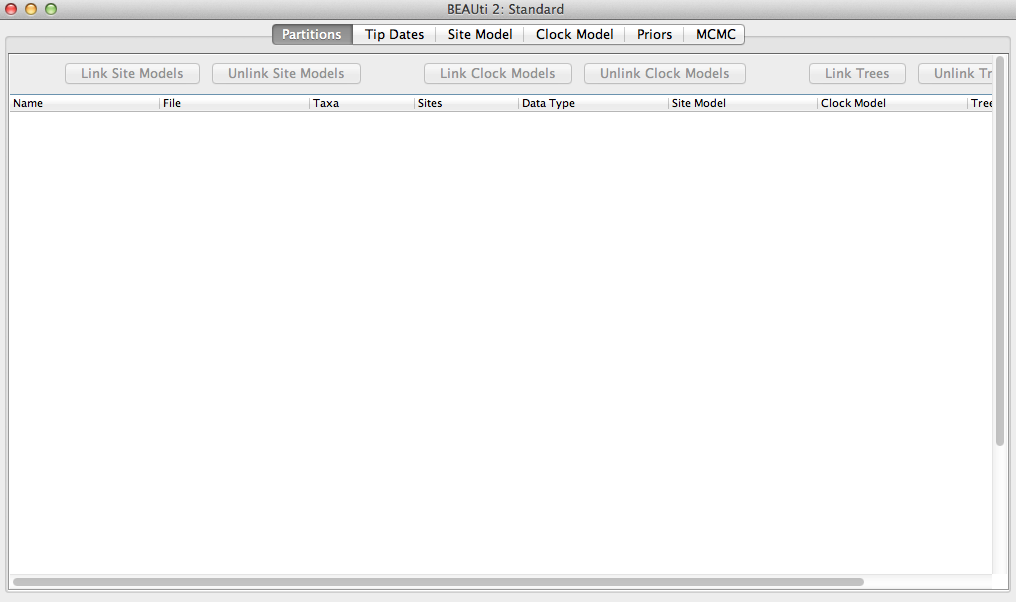
\includegraphics[width=0.7\textwidth]{../screenshots/beauti-init.png}}
        \caption{BEAUTi window launched from \program{BEAST}.}
        \label{fig:beautiInit}
    \end{figure}
}

\step{Install SNAPP and model selection packages}{We need to add functionality to \program{BEAST} in order to estimate 
     species trees with SNP data and 
     to perform model selection. Begin by using the drop-down 
     menu \subItem{File}{Manage Packages.} A window should 
     appear that looks something like Figure~\ref{fig:beauti-manage-packages}.
     Select and install the packages \program{{\bf SNAPP}} and \program{{\bf Model\_Selection}}. You can then exit the 
     window by clicking the {\bf ``Close''} button.
    \begin{figure}[htbp]
        \centering
        \fbox{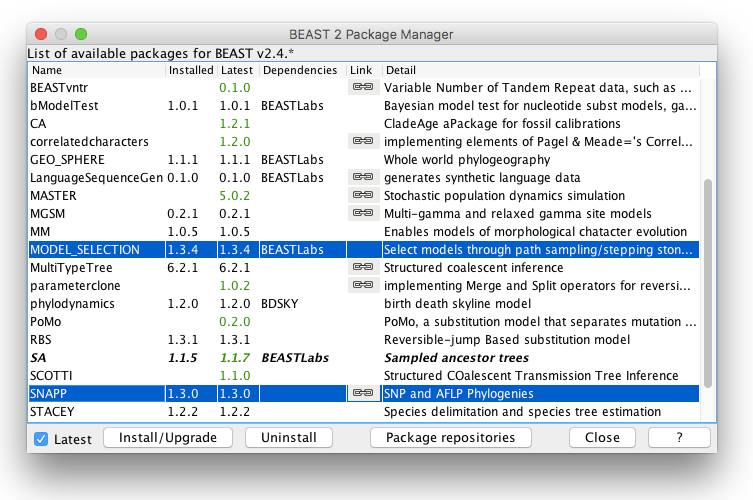
\includegraphics[width=0.7\textwidth]{../screenshots/beauti-manage-packages.png}}
        \caption{\program{BEAUTi} package manager for \program{BEAST}.}
        \label{fig:beauti-manage-packages}
    \end{figure}

}

\step{Converting \program{BEAUTi} to \program{SNAPP} mode}{We need to tell \program{BEAUTi} that we are 
     setting up a \program{SNAPP} analysis, which will change the menu options and allow us to import SNP data.
     Begin by using the drop-down 
     menu \subItem{File}{Template, SNAPP}. This should change the appearance of the \program{BEAUTi} 
     window to look something like Figure~\ref{fig:beauti-snapp}.

    \begin{figure}[htbp]
        \centering
        \fbox{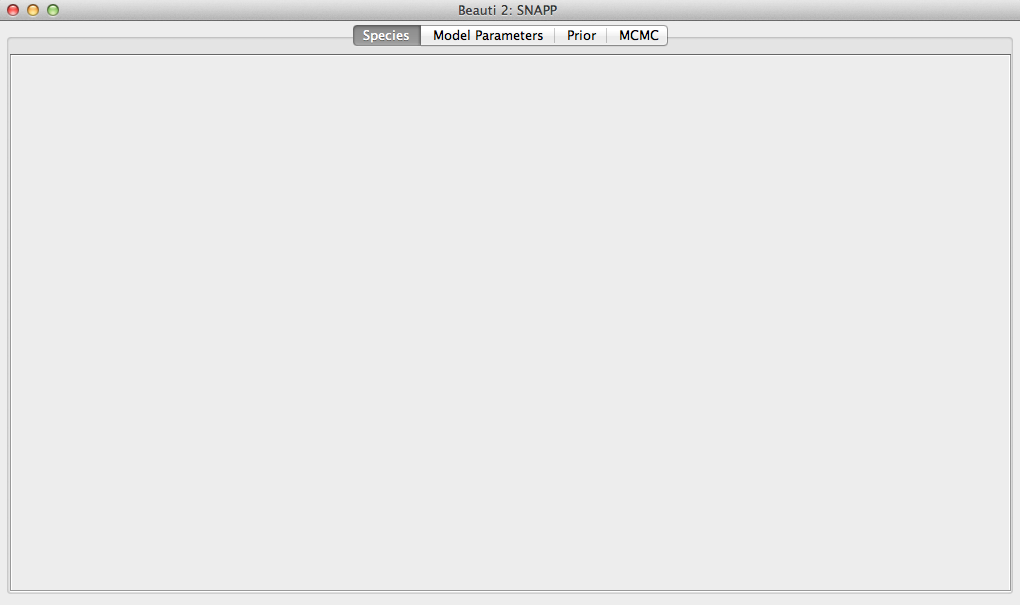
\includegraphics[width=0.7\textwidth]{../screenshots/beauti-snapp.png}}
        \caption{\program{BEAUTi} window after importing the \program{SNAPP} template. Notice that the menu tabs have changed.}
        \label{fig:beauti-snapp}
    \end{figure}

}


\step{Import the SNP data.}{
    Import the SNP data (the {\bf hemi129.nex} file)
    using the drop-down menu \subItem{File}{Import Alignment.}

    Once the data are successfully loaded into \program{BEAUTi} you should see a list of the 
    samples included in the data file (Figure~\ref{fig:beauti-data-imported}.)

    \begin{figure}[htbp]
        \centering
        \fbox{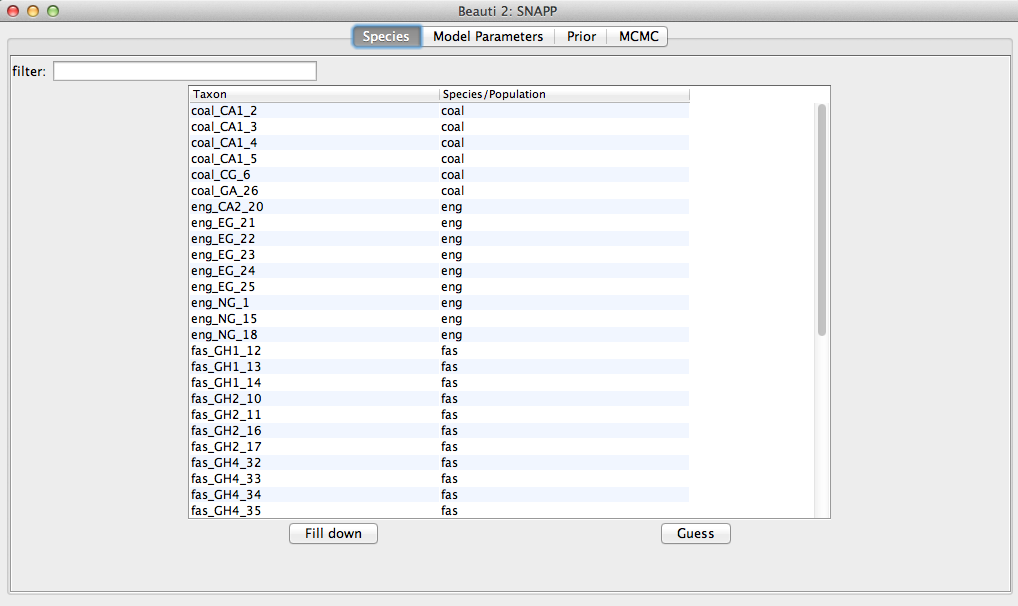
\includegraphics[width=0.8\textwidth]{../screenshots/beauti-data-imported.png}}
        \caption{The data successfully loaded by BEAUTi.}
        \label{fig:beauti-data-imported}
    \end{figure}
}

\step{Define species.}{
    There are several ways to designate species assignments. We automatically 
    designated species names using the names already 
    present in the data files. The species names can be pre-defined this way by including a ``delimiter'' that 
    allows the species name to be separated from the rest of the sequence name. The gecko data 
    file uses an underscore ``\_'' to separate
    the species name (on the left) from the rest of the sequence name (on the right) as follows:\\
    \\
    \cmd{eng\_NG\_1}\\ 	
    \cmd{coal\_CA1\_2}\\	
    \cmd{coal\_CA1\_3}\\
    \cmd{coal\_CA1\_4}\\	
    \cmd{coal\_CA1\_5}\\	
    \cmd{coal\_CG\_6}\\	
    \cmd{kya\_GH3\_7}\\	
    \cmd{kya\_GH3\_8}\\	
    \cmd{\ldots}\\
    \\
    Other options for assigning species names are available using the ``Guess'' button. The screen should look similar to 
     Figure~\ref{fig:beauti-guess-trait}. The original data include 46 samples, but the XML files included in this tutorial contain 
     a reduced number of samples to speed up the analyses.

    \begin{figure}[htbp]
        \centering
        \fbox{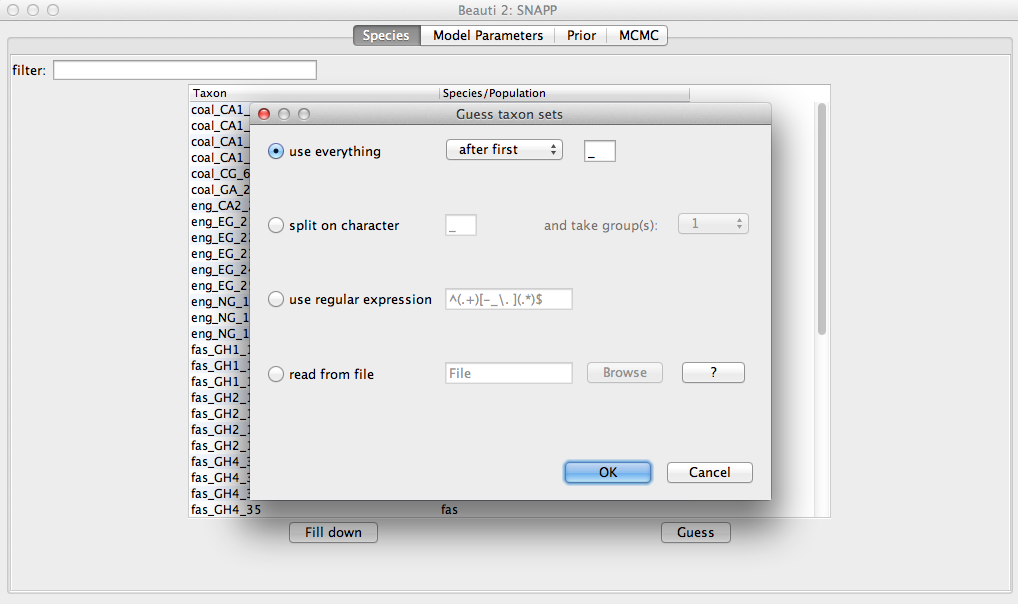
\includegraphics[width=0.8\textwidth]{../screenshots/beauti-guess-trait.png}}
        \caption{The species assignment options that appears after you select the ``Guess' button.}
        \label{fig:beauti-guess-trait}
    \end{figure}
 
    You can import a custom mapping file that links each sample to a species using the ``read from file'' option.      
    Click the ``Ok'' button to return to the \menutab{Species} window. Be sure that each Taxon has a Species/Population name.    
}


\step{Set the mutation model.}{
    Next, we need to set up our model under the \menutab{Mutation Model} tab Figure~\ref{fig:beauti-mutation}.
    We will use the default options for this tutorial, but you should read the documentation \href{http://www.beast2.org/wiki/index.php/SNAPP}{A rough guide to SNAPP} to learn more about the model options. Briefly, the parameters are as follows:

\small{
    \begin{compactdesc}
       \item[\field{Mutation Rate U: instantaneous rate of mutating from the 0 allele to the 1 allele.}]
       \item[\field{Mutation Rate V: instantaneous rate of mutating from the 1 allele to the 0 allele.}]
       \item[\field{Coalescence Rate: population size parameter with one value for each node in the tree.}]
    \end{compactdesc}
    
    The ``Include non-polymorphic'' checkbox is used in cases where invariant sites have been included in the data. The likelihood calculations are 
    different if \program{SNAPP} assumes that all constant sites have been removed.
    
    The ``Mutation Only At Root'' checkbox indicates conditioning on zero mutations, except at root (default false). As a result, all gene 
    trees will coalesce in the root only, and never in any of the branches.
    
    The ``Show Pattern Likelihoods And Quit'' checkbox is handy if you just want to print out the likelihoods for all patterns in the starting state and then quit.
    
    The ``Use Log Likelihood Correction'' checkbox is for calculating corrected likelihood values for Bayes factor test of different species assignments.
        
    }
    
        \begin{figure}[htbp]
        \centering
        \fbox{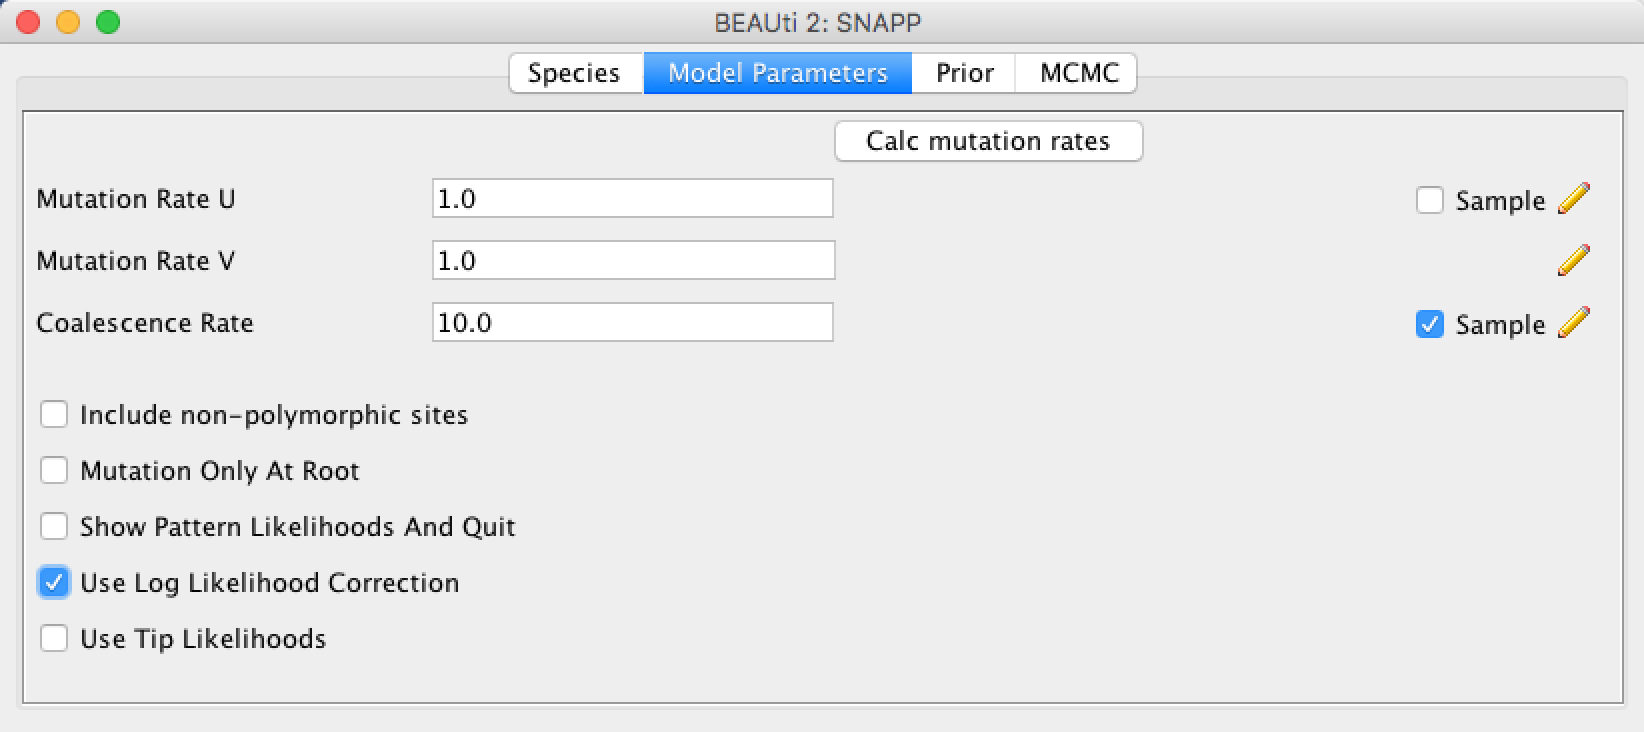
\includegraphics[width=0.8\textwidth]{../screenshots/beauti-mutation.png}}
        \caption{The Mutation Model options.}
        \label{fig:beauti-mutation}
    \end{figure}
}

    
\step{Define the priors.}{
    Next, we need to move to the \menutab{Prior} tab and specify the priors (Figure~\ref{fig:beauti-prior}.) We will use the 
    default options for this tutorial, but you should read the 
    documentation \href{http://www.beast2.org/wiki/index.php/SNAPP}{A rough guide to SNAPP} 
    to learn more about these options. A short description of the priors are provided below:
    Briefly, \program{SNAPP} uses a Yule prior for the species tree and branch lengths on the species tree. 
    This prior has a single parameter, {$\lambda$} (Lambda), which governs the rate that species diverge. This rate, in turn, determines the (prior) 
    expected height of the species tree. 
\small{
    \begin{compactdesc}
       \item[\field{Alpha: shape parameter for the gamma prior on population sizes.}]
       \item[\field{Beta: scale parameter for the gamma prior on population sizes.}]
       \item[\field{Kappa: parameter used when selecting the CIR rate prior (below).}]
       \item[\field{Lambda: Birth rate for the Yule model prior on the species tree.}]
       \item[\field{Rateprior: prior on rates can be Gamma, InverseGamma, CIR, or Uniform.}]
    \end{compactdesc}
}
    
    \begin{figure}[htbp]
        \centering
        \fbox{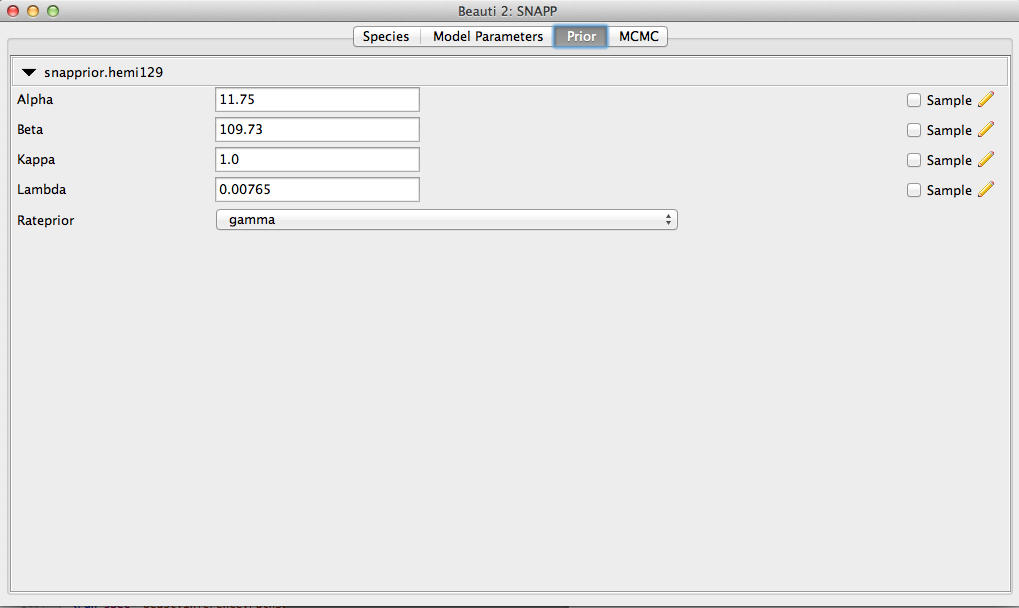
\includegraphics[width=0.8\textwidth]{../screenshots/beauti-prior.png}}
        \caption{The prior settings.}
        \label{fig:beauti-prior}
    \end{figure}   
    }


\step{Specify MCMC settings and generate the XML file.}{
    Next, move to the \menutab{MCMC} tab. 
    Change the following settings:
    \begin{compactdesc}
        \centering
        \item[\field{State Burnin:}] \fieldvalue{0}
        \item[\field{Chain Length:}] \fieldvalue{1000}
        \item[\field{Store Every:}] \fieldvalue{10}
        \item[\field{tracelog:File Name:}] \fieldvalue{runA.log}
        \item[\field{tracelog:Log Every:}] \fieldvalue{10}
        \item[\field{treelog:File Name:}] \fieldvalue{runA.trees}
        \item[\field{treelog:Log Every:}] \fieldvalue{10}
    \end{compactdesc}
    Leave the remaining options at their default values
    (Figure~\ref{fig:beauti-mcmc}). These MCMC values are way to low, and a thorough analysis requires much more computational time. 
    The original SNP data include 46 samples, but the files 
    included in this tutorial contain a reduced number of samples to speed up the analyses. 
    The MCMC run times are intentionally kept short (and the data files reduced) in this tutorial. These short analyses should run in approximately 2 -- 4 minutes depending
    on the number of processors available on your computer.  
    Thorough analyses of the full data take 2 -- 6 days, depending on the number of species in the model. A SNP matrix with 1,000 loci requires 5 -- 20 days.
 
    \begin{figure}[htbp]
        \centering
        \fbox{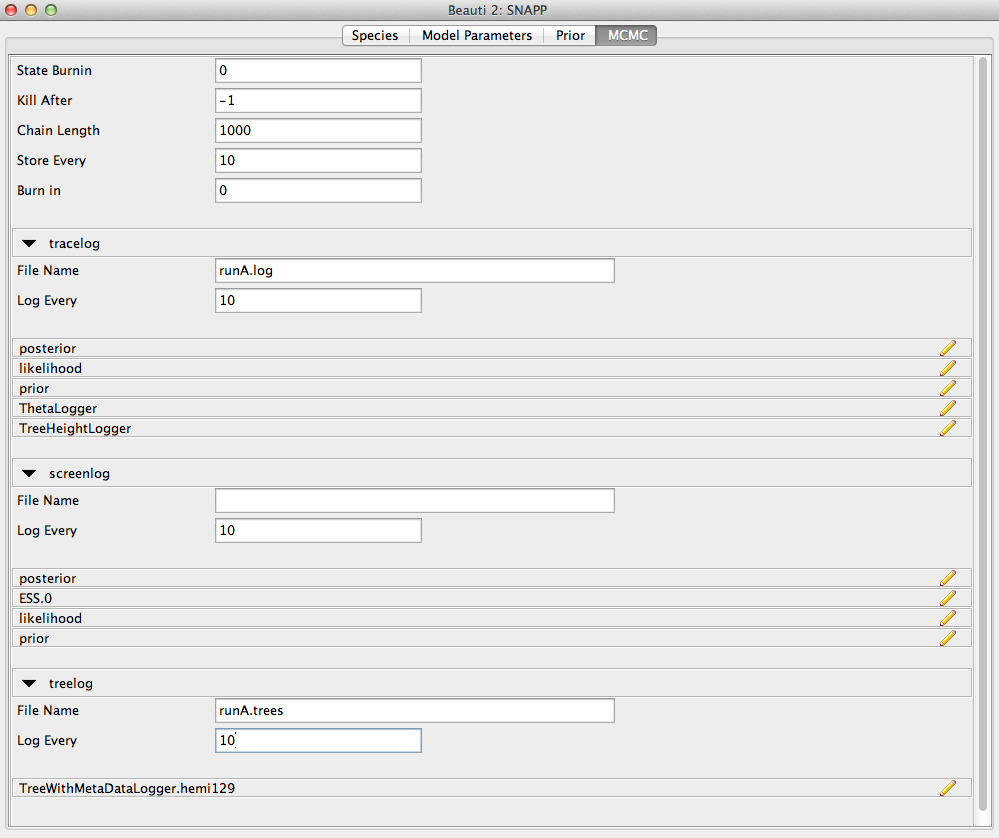
\includegraphics[width=1.0\textwidth]{../screenshots/beauti-mcmc.png}}
        \caption{The MCMC settings.}
        \label{fig:beauti-mcmc}
    \end{figure}

    Next, save the file using \subItem{File}{Save\ldots.} 
    Another subwindow will appear for specifying the name and location for
    saving the XML file. Name the file ``runA.xml'' and place it in a folder with the same name.
    Save the file to
    the \localfile{BFD*-tutorial} folder.\\
    }

\intermediate{\subsection{Editing the XML file for marginal likelihood estimation}}

\step{Editing the XML file for marginal likelihood estimation.}{
Species delimitation using SNPs requires marginal likelihood estimation. 
You will need to edit the XML file to prepare it for analysis in \program{BEAST}. Instructions for setting up
marginal likelihood estimation using path sampling are provided at the \href{http://www.beast2.org/wiki/index.php/Path_Sampling}{BEAST} website. The procedure involves (1) typing in some short codes in a few places, (2) replacing some words, and (3) copying and pasting some sections around.
 
Open your XML file in a text editor. Search and replace the opening run statement (located about half way through the file) with an mcmc statement by changing {\bf ``<run ...>''} into {\bf ``<mcmc ...>''.} Next, type a new closing mcmc statement, {\bf ``</mcmc>''}, just before the closing run statement, {\bf ``</run>''}, located at the end of the file.

Now you are ready to insert the path sampling commands. You will need to insert the following block of text into your XML file immediately above the opening ``<mcmc ...>''' element:

\small{
\cmd{<run spec=`beast.inference.PathSampler'}\\ 
\cmd{chainLength="1000"}\\
\cmd{alpha=`0.3'}\\
\cmd{rootdir=`/home/desktop/BFD*-tutorial/runA/'}\\
\cmd{burnInPercentage=`0'}\\
\cmd{preBurnin="0"}\\
\cmd{deleteOldLogs=`true'}\\ 
\cmd{nrOfSteps=`24'>}\\
\cmd{cd \$(dir)}\\
\cmd{java -cp \$(java.class.path) beast.app.beastapp.BeastMain \$(resume/overwrite) -java -seed \$(seed) beast.xml}\\
}


{\bf Important:} If you copy and paste this section into your XML file, be sure to check that the symbols paste correctly. The quote symbols (`` ` ' ") don't copy as they should, and these will cause problems. Also, make sure that the root directory path (rootdir) exists on your computer.

	These path sampling parameters are way to low, and a thorough analysis requires much more computational time. The MCMC run times are 
    intentionally kept short in this tutorial so that we have time to conduct analyses and discuss the results.

The path sampling parameters that you just entered into your XML file are as follows:

    \begin{compactdesc}
       \item[\field{chainLength: MCMC sample length for each path sampling step.}]
       \item[\field{alpha: parameter used to space out path sampling steps.}]
       \item[\field{rootdir: directory for storing output. Be sure that the folder exists before starting the run.}]
       \item[\field{burnInPercentage: burn-In percentage used for analyzing the log files.}]
       \item[\field{preBurnin: number of samples that are discarded for the first step, but not the others.}]
       \item[\field{deleteOldLogs: delete existing log files from rootdir}]
      \item[\field{nrOfSteps: the number of path sampling steps to use}]
    \end{compactdesc}
    
For older versions of \program{SNAPP} (<v1.1.10) you may need an extra step; find the text {\bf ``snap.MCMC''} and replace it with {\bf ``beast.core.MCMC''.}  
Finally, move the entire {\bf ``stateDistribution''} element to just before the run element. This step requires that you move all of the lines starting with {\bf ``<stateDistribution''} and ending with {\bf ``</stateDistribution>''} to just above the run element.


}

        
\intermediate{\subsection{Running the XML file with \program{BEAST}}}

\step{Run the XML file in \program{BEAST.}}{
	    You can execute the XML file in \program{BEAST} using the GUI or the command line. If you are using Mac OSX or Windows, you should 
	    be able to do launch the \program{BEAST} GUI by double clicking on the application icon. 
	    After the \program{BEAST} window appears, click the \field{Choose File\ldots} button, 
	    and select the XML file you just created (Figure~\ref{fig:beast}). Increase the \field{Thread pool size} to the 
	    maximum number of threads that you can run on your computer. 
	    Click \field{Run}. The analysis should take about 10 minutes. 
	    You can also run \program{BEAST} from the command line. Open the {\bf Terminal} Application and navigate to the folder 
	    containing your {\bf runA.xml} file. To execute the file, type the following at the command line:
	    
	    \cmd{/path/to/BEASTv2.1.2/bin/beast -threads 8 runA.xml}
	    
	    or
	    
	    \cmd{beast -threads 8 runA.xml}
	    
	    if you have already moved the \program{BEAST} executable to your path. Remember to set the number of \field{threads} to the maximum number available on your computer.
	  
	
	\begin{figure}[htbp]
        \centering
        \fbox{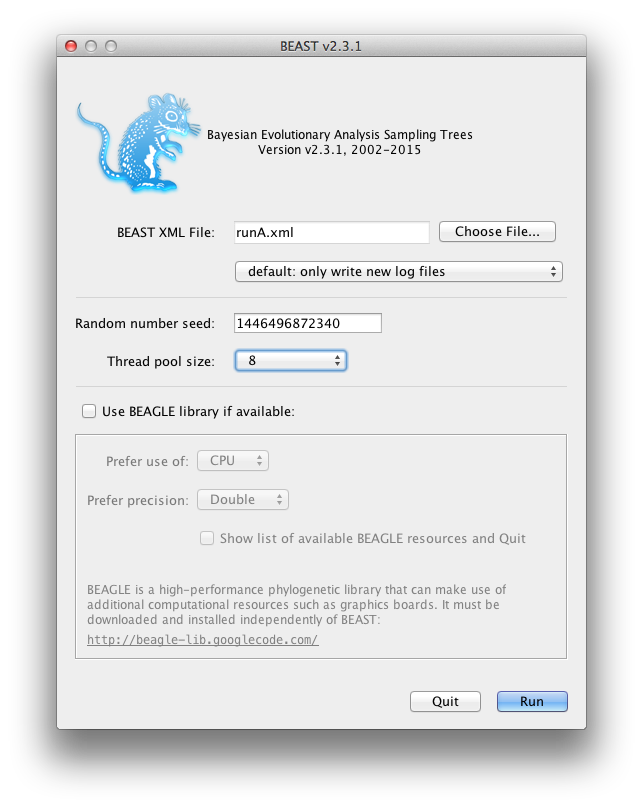
\includegraphics[width=0.5\textwidth]{../screenshots/beast.png}}
        \caption{The \program{BEAST} GUI window.}
        \label{fig:beast}
    \end{figure}
    }

\intermediate{\subsection{Inspecting path sampling results}}

\step{Inspecting path sampling results.}{
At the end of your analysis, the path sampling results will be displayed on the screen. An example is shown in Figure~\ref{fig:beast-output}. 
Each row shows the results from one path sampling step. The example in Figure~\ref{fig:beast-output} shows the results from a path sampling analysis with 24 steps. You will use the value after "marginal L estimate" to compare models. 

       \begin{figure}[htbp]
        \centering
        \fbox{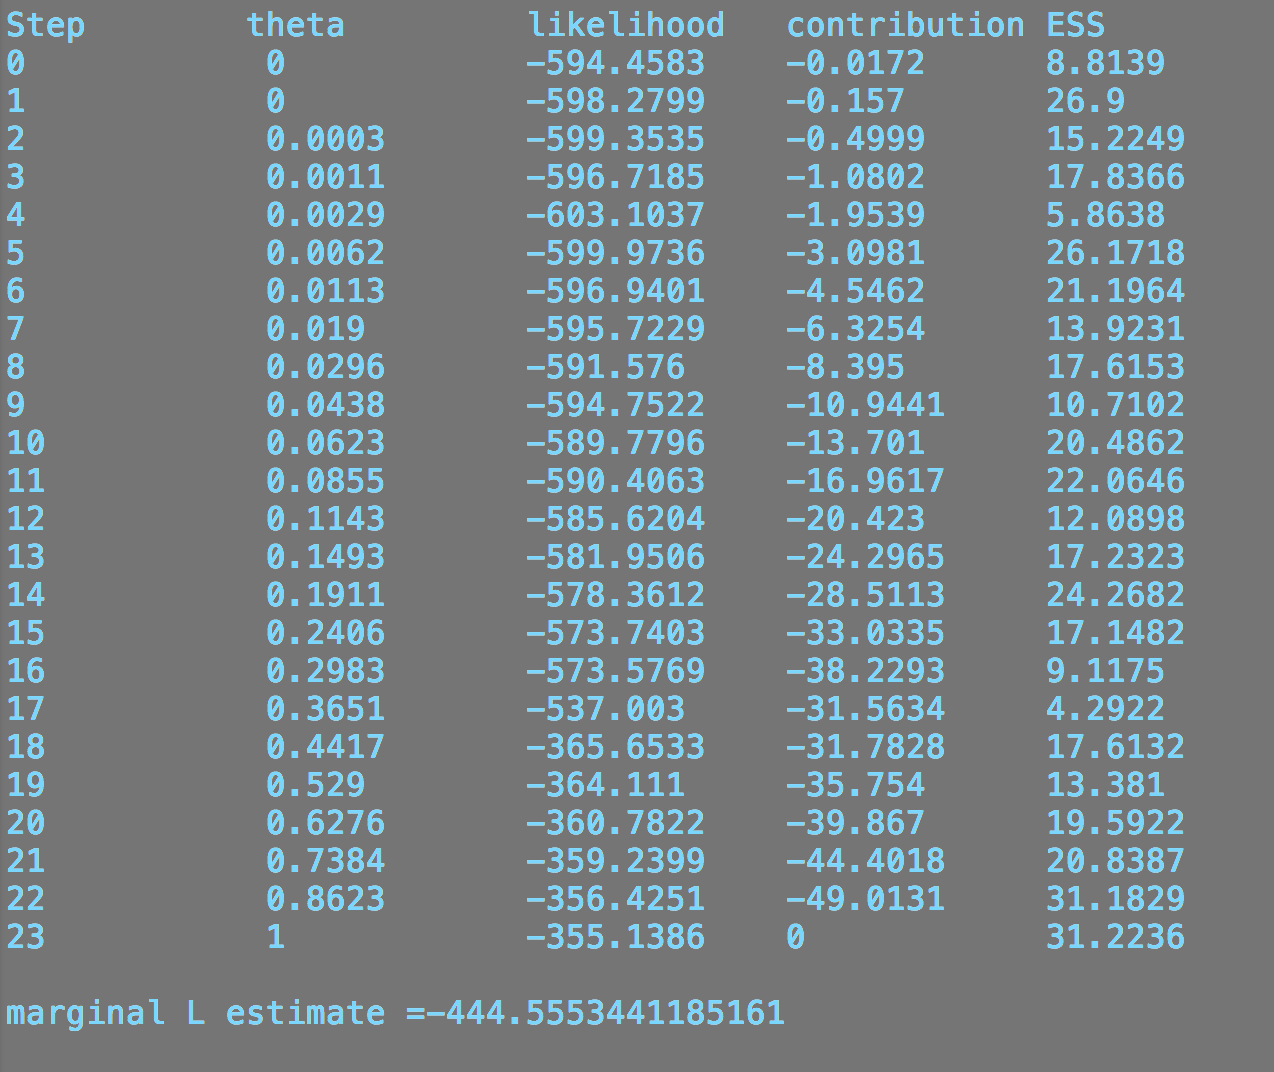
\includegraphics[width=0.5\textwidth]{../screenshots/beast-output.png}}
        \caption{The path sampling output at the end of the analysis.}
        \label{fig:beast-output}
    \end{figure}
}



\intermediate{\subsection{Setting up new species delimitation models}}

\step{Setting up new XML files for species delimitation.}{
Now that you have one XML file up and running it is easy to make new XML files for each species delimitation model.
To prepare a new file for species delimitation, we
have to make a few slight modifications to the existing runA.xml file: (1) save a copy of the xml file as runB.xml and save it in a new folder with the same name, (2) change the file stem names in the xml file so that you don't accidentally overwrite any of your previous results, (3) edit the path sampling root directory to point to the new runB folder, 4) change the species assignments listed in the  {\bf ``stateDistribution''} element. This last part requires changing the number and/or composition of taxonset features. Each taxonset begins with {\bf ``<taxonset ...>''} and ends with {\bf ``</taxonset>''} (Figure~\ref{fig:beast-taxon-set}). To lump species, simply combine the taxon names into a single  taxonset feature. To split a species, simple create a new taxonset containing the appropriate taxon names. To reassign a taxon to a different species you can cut and paste the taxon to the new taxonset. 
XML files containing the species assignments shown in Figure \ref{fig:map} are provided with this tutorial (see Box~\ref{box:tutorialDir}). The XML files included with this tutorial contain a reduced number of samples in the taxonset blocks to help speed up the analyses.

       \begin{figure}[htbp]
        \centering
        \fbox{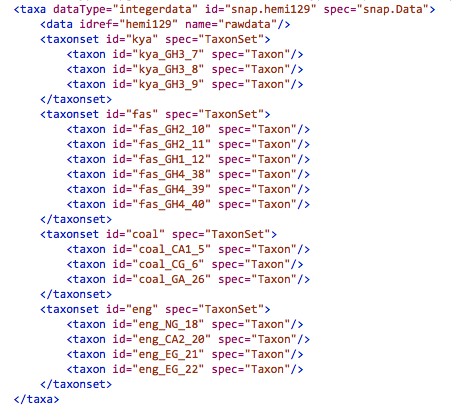
\includegraphics[width=0.5\textwidth]{../screenshots/beast-taxon-set.png}}
        \caption{Example of the taxonset features in the XML file.}
        \label{fig:beast-taxon-set}
    \end{figure}
}


\step{Comparing species delimitation models with Bayes factors.}{  
   After you run each of the alternative species delimitation models you can rank them by their marginal likelihood estimate (MLE). You 
   can also calculate Bayes factors to compare the models. 
   The Bayes factor (BF) is a model selection tool that is simple and well suited for the purposes of comparing species delimitation models. 
   Calculating the BF between models is simple. To do so, simply subtract the MLE values for two models, and then multiply the difference by two (BF = 2 x (model1 - model2). A negative BF value indicates support in favor of model 1. A positive BF value indicates support in favor of model 2. 

The strength of support from BF comparisons of competing models can be evaluated using the framework of \cite{kass95}. 
 The BF scale is as follows: 
0 < BF < 2 is not worth more than a bare mention, 2 < BF < 6 is positive evidence, 6 < BF < 10 is strong support, and BF > 10 is decisive.

The results for the seven gecko models are provided in Table 1. The model that splits \textit{Hemidactylus eniangii} into two species (runF) is the top-ranked model. It has the largest MLE value, and it is supported in favor of the current taxonomy model (runA). The BF in support for model F is decisive compared to model A. 

Table 1: Path sampling results for the seven species delimitation models shown in Figure \ref{fig:map}.
\begin{table}[ht]
\tabcolsep=0.2cm
\begin{tabular}{l c c c c } 
\hline     
Model 							& Species 	& MLE 	& Rank 	& BF\\\hline
runA, current taxonomy				& 4 			& -1673.4 	& 2		& -- \\
runB, lump western forests			& 3 			& -1724.2 	& 5		& +101.5\\
runC, lump central forests				& 3 			& -1788.0 	& 6		& +229.2\\
runD, lump western \& central forests	& 2 			& -1842.9 	& 7		& +339.0\\
runE, split \textit{fasciatus}			& 5 			& -1713.2 	& 4		& +79.7\\
runF, split \textit{eniangii} 				& 5 			& -1625.9 	& 1		& -95.1 \\
runG, reassign Bioko Island			& 4 			& -1712.6 	& 3 		& +78.4\\\hline
\end{tabular}\\
MLE = Marginal likelihood estimate\\
BF = Bayes factor\\
\end{table}
}

\intermediate{\subsection{Summarizing the trees using \program{TreeAnnotator}.}}

\step{Summarize the species tree using \program{TreeAnnotator}.}{
TreeAnnotator will summarize the posterior distribution of species trees and identify the topology with the best posterior support, and summarize the divergence times for each node in the tree.
	Launch the \program{TreeAnnotator} program.
    You can also specify the burnin value if you haven't already excluded burn-in samples in \program{LogCombiner}.
	For the \field{Target tree type} field, choose \fieldvalue{Maximum clade credibility tree}.
    For the \field{Node heights} field, choose \fieldvalue{Median heights}.
	Select the \field{Input Tree File} button and select the file \localfile{runA.trees}.
	Select the \field{Output File} button and specify the \localfile{output} directory and a 
	file name, \localfile{runA-MCC.tre}.
	Click \field{Run}
}

\intermediate{\subsection{Visualizing the tree in \program{FigTree}}}

\step{Visualize the species tree in \program{FigTree}.}{
    Launch the \program{FigTree} program, and load the \localfile{runA-MCC.tre} file
    you just created with \program{TreeAnnotator}.
    Check the \field{Branch Labels} option and select
    \fieldvalue{posterior} for the \subItem{Branch labels}{Display} fields.
    Check the \field{Node Bars} option and select
    \fieldvalue{height\_95\%\_HPD} for the \subItem{Node bars}{Display} field.
    
}




